\section{Fundamentals and Related Work} \label{fundamentals_related_work}

Q-learning is a known off-policy and model-free approach to train an agent based on temporal difference in an environment that can be modeled as a Markov Decision Process (MDP). An agent therefore does not necessarily use the policy it is trained for and does not know the transition probabilities and rewards in the MDP beforehand. \autoref{QLearning} shows the iterative update formula for the Q-values that an online model uses to choose the right action \cite{Geron2018}.

\begin{equation} \label{QLearning}
	Q_{k+1}(s,a) = (1-\alpha) Q_k(s,a) + \alpha(r + \gamma \max_{a'} Q_k(s',a')) 
\end{equation}

The problem with conventional Q-learning is that in most of the cases the state dimension is far too high to explore and model the MDP entirely in foreseeable future. To deal with this problem the Q-values need to be approximated using a regression model. Deep neural networks have proven to be highly applicable for this task, which leads to the term of \textit{Deep Q-learning} and respectively \textit{Deep Q-Networks} (DQN) for such network architectures. DQNs use the vectorized numerical state as its input and outputs the predicted Q-values. It learns through backpropagating the temporal difference error over each step for a single neuron. Note that for the Q-learning algorithm a backpropagation is done after every step of the simulation. To avoid temporal correlation between succeeding experiences an experience replay buffer is used to randomly sample a training batch in each step. Also rare experiences will be used more frequently to update the model parameters using this approach. In the following papers regarding DQN architectures shall be introduced as well as papers dealing with the bomberman environment for Reinforcement Learning. 

Paper \cite{vanHasselt2015} tackles the problem that the $max$ operator in \autoref{QLearning} often leads to overoptimistic value estimates as the DQN uses the same Q-values to both select and evaluate an action. It therefore changes the iterative update formula to \ref{DoubleQLearning}.

\begin{equation} \label{DoubleQLearning}
	Q_{k+1}(s,a) = (1-\alpha) Q_k(s,a) + \alpha(r + \gamma Q'_k(s', arg\max_{a'} Q_k(s',a'))) 
\end{equation}

Now a target DQN is used to separate the determination of the greedy policy, which is still done by the online network, from the Q-value estimation. Using this double DQN approach results in less overestimated Q-values and therefore better policies by more accurate Q-value estimates. It also makes the learning process more stable and reliable. The weights are copied from the online network to the target network after a fixed amount of episodes.

Another optimization was introduced in paper \cite{Wang2016}. It changes the architecture of the DQN by splitting it into two separate value streams. One stream estimates the state value function and the other one the state-dependent action advantage function. Both streams are then combined again using a special aggregating layer to produce an estimate of the Q-values (see \autoref{fig:duelingDQN}).  

\begin{figure}[ht]
	\centering
	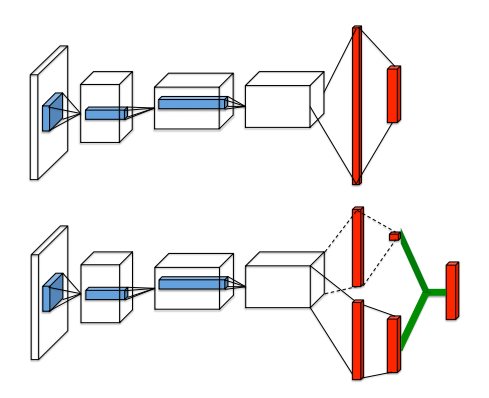
\includegraphics[width=0.6\linewidth]{figures/duelingDQN.PNG}
	\caption{Architecture of a normal DQN (top) compared to a dueling DQN (bottom)}
	\label{fig:duelingDQN}
\end{figure}

The state-dependent action advantage function is defined as

\begin{equation} \label{advfunction}
	A^{\pi}(s,a) = A^{\pi}(s,a) - V^{\pi}(s)
\end{equation}

and measures the importance of each action. The special aggregating layer uses \autoref{aggregation} to estimate the Q-values while also tackling the issue of identifiability. 

\begin{equation} \label{aggregation}
	Q(s, a; \theta, \alpha, \beta) = V(s; \theta, \beta) + (A(s, a; \theta, \alpha) - \frac{1}{\abs{A}} \sum_{a'}A(s, a'; \theta, \alpha)) 
\end{equation}

Using the dueling architecture approach an agent can learn which states are valuable independently of each action, which is especially useful in case actions do not influence the environment in any useful way. This leads to a better and more robust policy evaluation in the presence of many similar-valued actions. Also when looking at the last layer of a conventional DQN (see \autoref{fig:duelingDQN}) it usually becomes much more sparse and biased. As the state value is modeled as a single neuron in the dueling architecture, learning the state value function becomes much more efficient. 

Obviously, approaches exist that combine double Deep Q-learning with dueling architectures like \cite{Huang2018}. 

Besides optimizing the learning process itself and the model architecture, \cite{Schaul2016} now proposes a way to sample more efficiently from the experience replay buffer. Each experience is assigned a learning priority score $p_i$ with 

\begin{equation} \label{prio}
	p_i = \frac{1}{rank(i)}
\end{equation}

where $rank(i)$ is the rank of experience $i$ in the priority queue built upon the magnitude of the temporal difference error $\delta$ of each experience. The stochastic sampling probability of each experience is then calculated according to 

\begin{equation} \label{prob}
	P(i) = \frac{p_i^{\alpha}}{\sum_k p_k^{\alpha}} \;\;\;\; with \; 0\le\alpha\le1.
\end{equation}

The hyperparameter $\alpha$ determines the degree of using prioritization over random sampling. Using this stochastic sampling approach tackles the problem of a diversity loss and subsequent over-fitting when just greedyly sampling according to the magnitude of $\delta$. One could also choose 

\begin{equation} \label{prio2}
	p_i = \abs{\delta_i} + \epsilon
\end{equation}

instead of \ref{prio} but the latter is more prone to outliers. Furthermore, each gradient descent step during backpropagation needs to be weighted with 

\begin{equation} \label{weight}
	w_i = ( \frac{1}{N} \frac{1}{P(i)} )^\beta
\end{equation}

to counter a bias towards high prioritized experiences introduced using the prioritized experience replay buffer. The weights should also be normalized with $\frac{1}{max_i w_i}$. As an unbiased nature of weight updates is especially important during the last training updates near convergence, $\beta$ increases slowly from a start value $\beta_0$ to 1 over time. 

There are several other improvements mentioned in the rainbow paper \cite{Hessel2017} like multi-step learning, distributional Reinforcement Learning and noisy nets, but these are out of the scope for this small research project. 

Other papers were found that explicitly use DQNs within the Bomberman environment. One of them being \cite{Kormelink2018} which introduces two novel exploration strategies, Error-Driven-$\epsilon$ and Interval-Q, and compares them to conventional exploration strategies like Diminishing $\epsilon$-Greedy and Max-Boltzmann, whereas Max-Boltzmann with decreasing temperature parameter still performs best in the long run by empirical evaluation. Nevertheless Error-Driven-$\epsilon$, despite being less stable, learns faster than all other exploration techniques. The paper also gives an approach to encode the state. Therefore, the playing field is encoded by four matrices, which are computed as:

\begin{itemize}
	\item Free, breakable and obstructed cells are encoded as either 1, 0 or -1,
	\item The position of the player is encoded as 1, free cells as 0,
	\item The position of opponent players are also encoded as 1, free cells as 0 and
	\item The danger score for each cell is calculated as $\frac{time passed}{time needed to explode}$, which gets an additional negative sign in case a bomb was planted by the player itself.
\end{itemize}

The paper also gives valuable insights into the configuration of hyperparameters, rewards and the amount of training needed until convergence, which is about 100 generations à 10.000 episodes. 

\cite{Franca2019} uses an imitation-based learner that trains its model with the actor-critic proximal-policy optimization method in the Bomberman environment. Here insights about how rewards need to be chosen and which state representation to choose can also be derived. 

Bomberman seems to provide a perfect environment to try out different Reinforcement Learning methods, which is why \cite{daCruzLopes2016} provided an artificial intelligence platform around Bomberman including several associated intelligent agents and empirical experiments. 
